\subsection*{题目背景}

在T市有很多个酒店,这些酒店对于不同种类的食材有不同的需求情况,莱莱公司负责每天给这些酒店运输食材。

由于酒店众多,如何规划运输路线成为了一个非常重要的问题。你作为莱莱公司的顾问,请帮他们解决这个棘手的问题。


\subsection*{题目描述}

T市有 $N$ 个酒店,这些酒店由 $N-1$ 条双向道路连接,所有酒店和道路构成一颗树。不同的道路可能有不同的长度,运输车通过该道路所需要的时间受道路的长度影响。

在T市,一共有 $K$ 种主流食材。莱莱公司有 $K$ 辆车,每辆车负责一种食材的配送,不存在多辆车配送相同的食材。

由于不同酒店的特点不同,因此不同酒店对食材的需求情况也不同,比如可能 $1$ 号酒店只需要第 $1,5$ 种食材, $2$ 号酒店需要全部的 $K$ 种食材。

莱莱公司每天给这些公司运输食材。对于运输第 $i$ 种食材的车辆,这辆车可以从任意酒店出发,然后将食材运输到所有需要第 $i$ 种食材的酒店。假设运输过程中食材的装卸不花时间,运输车足够大使得其能够在出发时就装满全部所需食材,并且食材的重量不影响运输车的速度。

为了提高配送效率,这 $K$ 辆车可以从不同的酒店出发。但是由于T市对于食品安全特别重视,因此每辆车在配送之前需要进行食品安全检查。鉴于进行食品安全检查的人手不足,最多可以设置 $M$ 个检查点。

现在莱莱公司需要你制定一个运输方案:选定{\heiti{不超过}} $M$ 个酒店设立食品安全检查点,确定每辆运输车从哪个检查点出发,规划每辆运输车的路线。

假设所有的食材运输车在进行了食品安全检查之后同时出发,请制定一个运输方案,使得所有酒店的等待时间的最大值最小。酒店的等待时间从运输车辆出发时开始计算,到该酒店所有需要的食材都运输完毕截至。如果一个酒店不需要任何食材,那么它的等待时间为 $0$ 。


\subsection*{输入格式}

从标准输入读入数据。

输入的第一行包含 $3$ 个正整数 $N,M,K$ ($1 \le N \le 10^{2}, 1 \le M \le K \le 10$),含义见题目描述。

接下来 $N$ 行,每行包含 $K$ 个整数。每行输入描述对应酒店对每种食材的需求情况, $1$ 表示需要对应的食材, $0$ 表示不需要。

接下来 $N-1$ 行,每行包含 $3$ 个整数 $u, v, w$ ,表示存在一条通行时间为 $w$ 的双向道路连接 $u$ 号酒店和 $v$ 号酒店。保证输入数据是一颗树,酒店从 $1$ 编号到 $N$ ,保证 $1 \le u,v \le N$ 并且 $1 \le w \le 10^{6}$。


\subsection*{输出格式}

输出到标准输出。

输出一个整数,表示在你的方案中,所有酒店的等待时间的最大值。

\examplebox*{\lstinputlisting[frame=none]{data/21/4-1.in}}{\lstinputlisting[frame=none]{data/21/4-1.out}}

\begin{figure}[H]
    \centering
    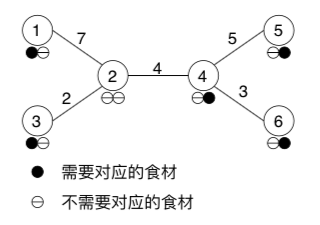
\includegraphics[width=0.6\textwidth]{image/21/4-p-1.png}
\end{figure}

样例1的输入数据如上图。由于限制了最多只能设置 $1$ 个检查点,因此可以设置两辆运输车的路径如下:

\begin{figure}[H]
    \centering
    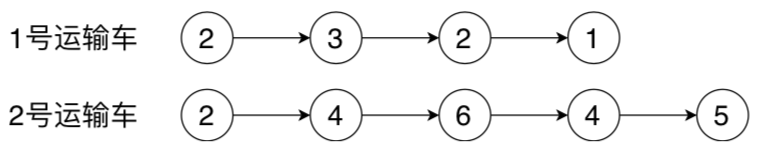
\includegraphics[width=0.9\textwidth]{image/21/4-p-2.png}
\end{figure}

在 $2$ 号酒店设置检查点,最晚拿到所有食材的酒店为 $3$ 号酒店,等待时间为 $9$。

\examplebox*{\lstinputlisting[frame=none]{data/21/4-2.in}}{\lstinputlisting[frame=none]{data/21/4-2.out}}

样例2的输入数据和样例1几乎完全相同,唯一的区别在于样例2中允许最多设置 $2$ 个检查点。我们可以设置两辆运输车的路径如下:

\begin{figure}[H]
    \centering
    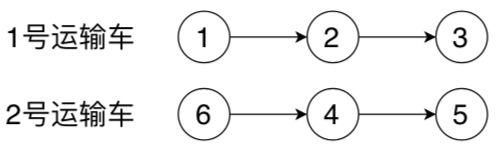
\includegraphics[width=0.9\textwidth]{image/21/4-p-3.png}
\end{figure}

在 $1$ 号酒店和 $6$ 号酒店设置检查点,最晚拿到所有食材的酒店为 $5$ 号酒店,等待时间为 $15$。

\subsection*{子任务}

本题目数据规模如下:

\begin{table}[H]
    \centering
    \begin{tabular}{c|c|c|c|c}
        \thickhline
        分数占比 & $N$                         & $M$                   & $K$                       & 特殊性                           \\ \hline
        $30\%$   & \multirow{3}{*}{$\le 10^2$} & \multirow{2}{*}{$=K$} & \multirow{3}{*}{$\le 10$} & 保证输入数据是一条链,且 $u+1=v$ \\ \cline{1-1} \cline{5-5}
        $40\%$   &                             &                       &                           & \multirow{2}{*}{无}              \\ \cline{1-1} \cline{3-3}
        $30\%$   &                             & $\le k$               &                           &                                  \\ \thickhline
    \end{tabular}
\end{table}